\section{Results with Asimov dataset for inclusive fiducial cross section measurements}

\begin{figure}[!h!t]
  \begin{center}  
    \subfigure[$\Hllll$]{
      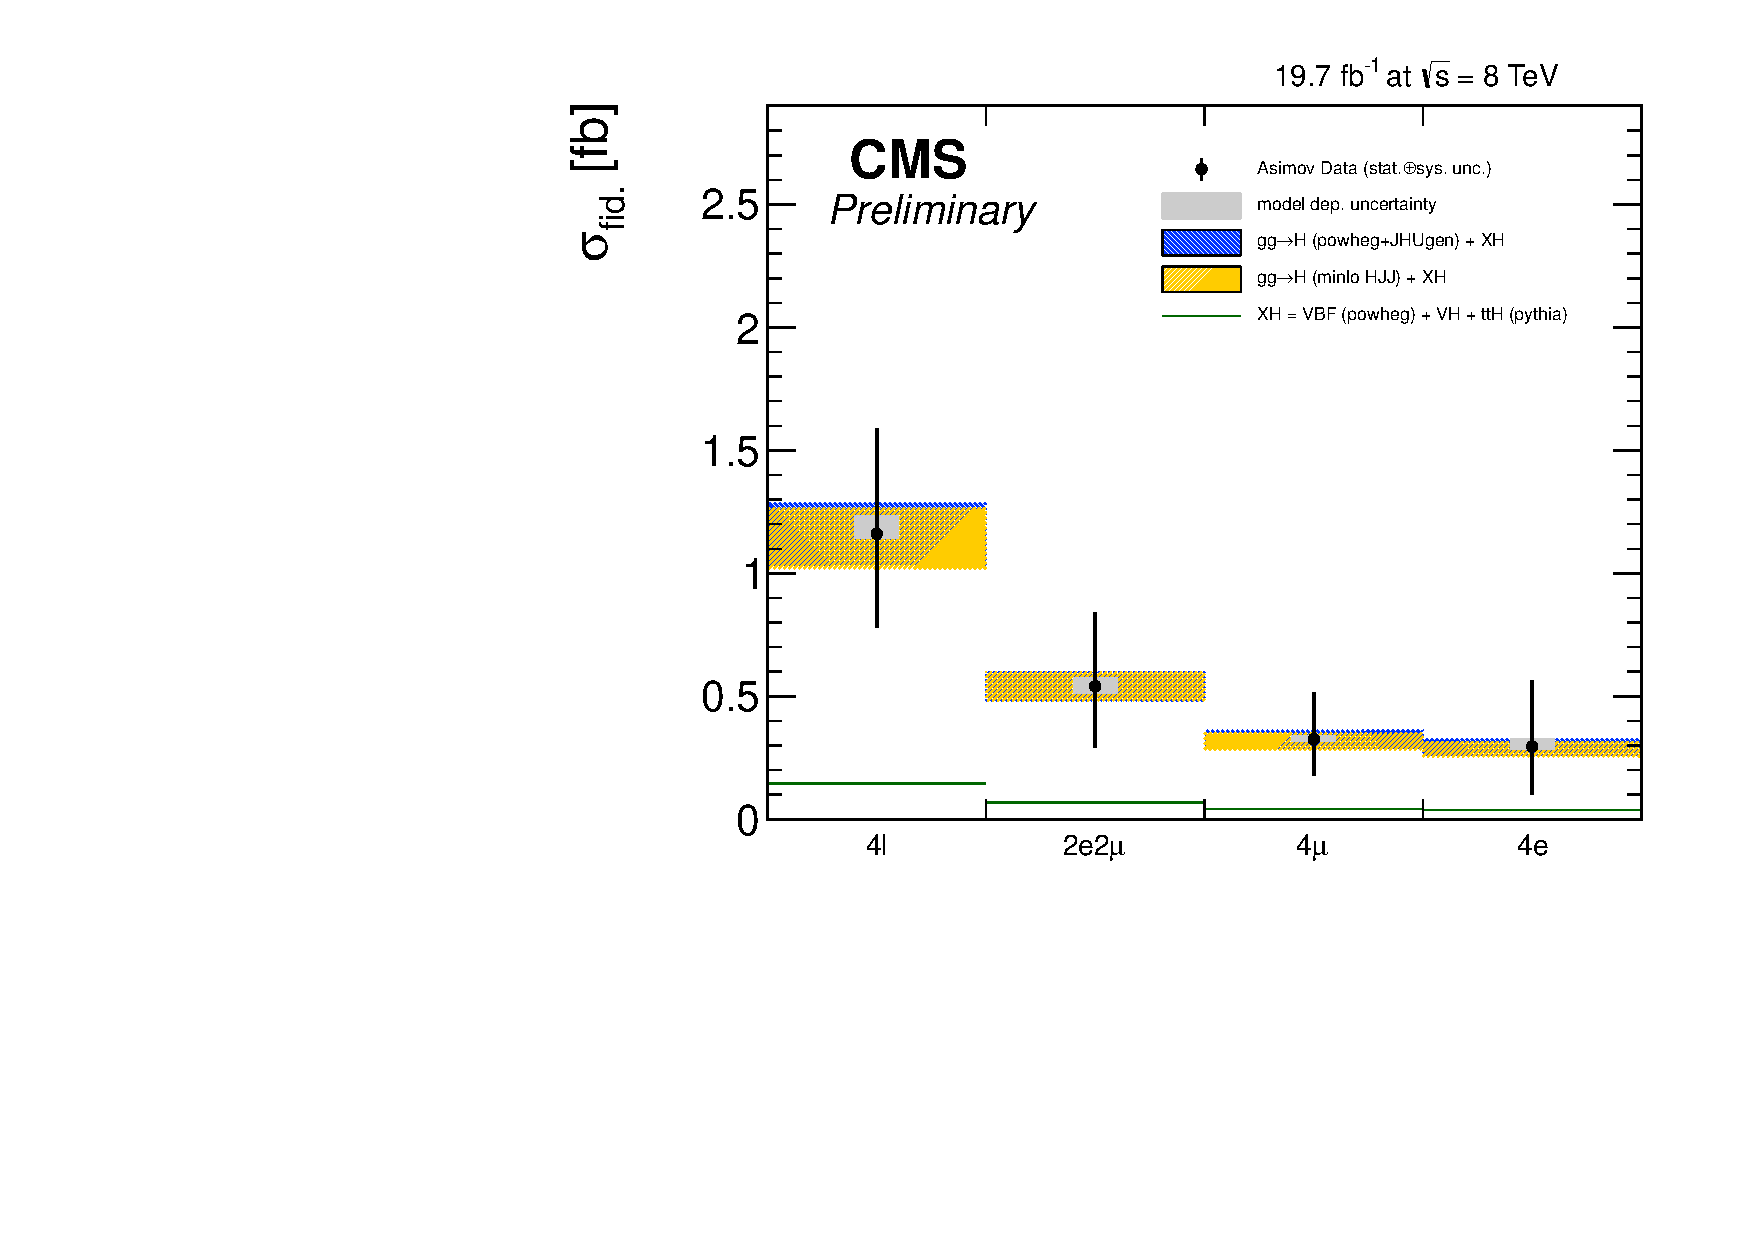
\includegraphics[width=0.48\textwidth,angle=0]{Appendix/Plots/mass4l_unfoldwith_SM_125.pdf}
      \label{fig:inclusive-results-asimov:a}
    }
    \subfigure[$\Zllll$]{
      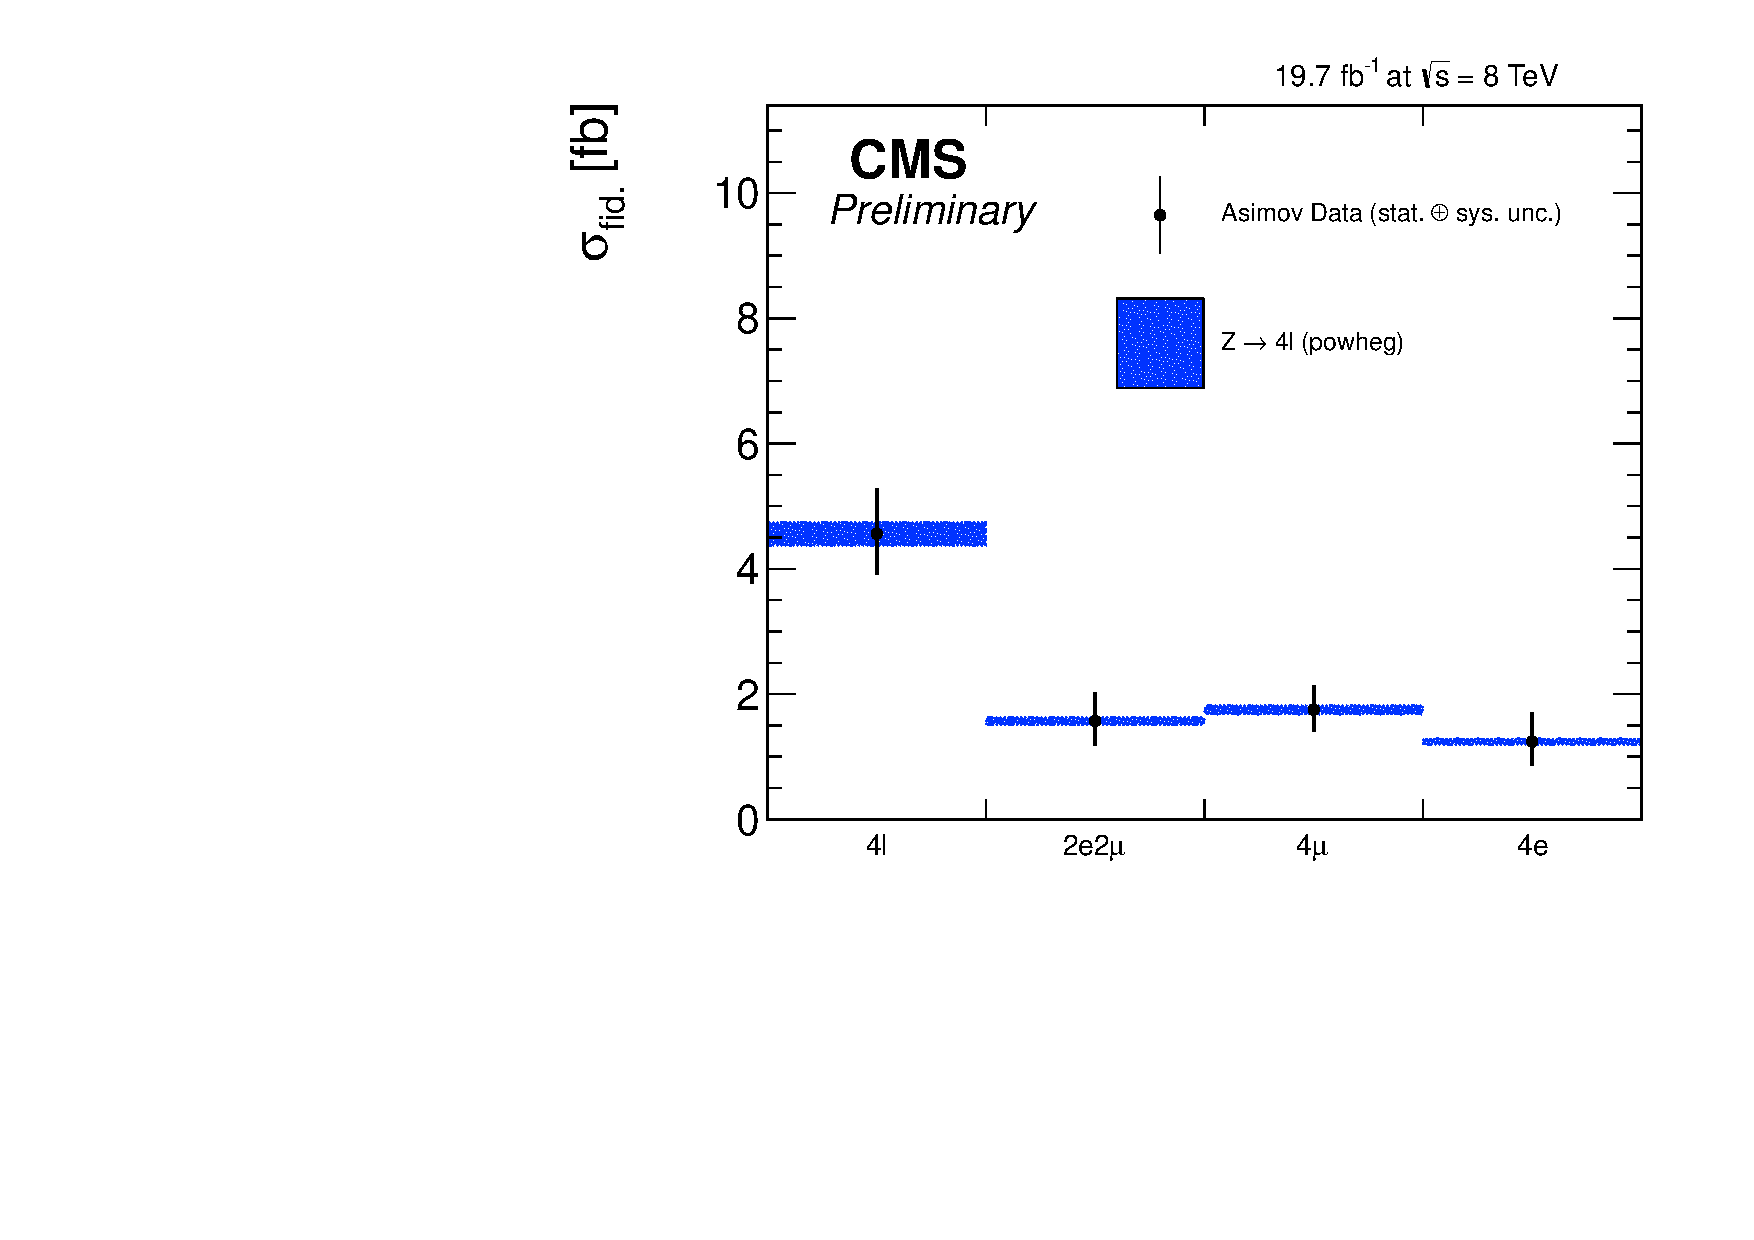
\includegraphics[width=0.48\textwidth,angle=0]{Appendix/Plots/fidxs_Z4l_SMZ4l_mass4l_Asimov_floatPOIs_fixMZ_all_8TeV_xs_v3_v2.pdf}
      \label{fig:inclusive-results-asimov:b}
    } 
    \caption{Results of the inclusive fiducial cross section measurement for different final states. 
    Predictions from {\sc powheg+JHUgen} and {\sc minloHJJ} are shown in blue and yellow, respectively.
    In case of the the total inclusive cross section measurement ($4\ell$, first bin) the fraction of $4e,4\mu,$ and $2e2\mu$ is floated in the fit.
    COMMENT: Results shown with Asimov dataset.
    } 
  \label{fig:inclusive-results-asimov}
 \end{center}
\end{figure}

%============
\begin{table}[!h!tb]
\begin{center}
      \caption{
The results of the $\Hllll$ inclusive fiducial cross section measurement performed in the $m_{4\ell}$ range from 105~GeV to 140~GeV, and
results of the $\Zllll$ inclusive fiducial cross section measurement performed in the $m_{4\ell}$ range from 50~GeV to 105~GeV.
    COMMENT: Results shown with Asimov dataset.
        } \label{tab:incresultsPAS-asimov}
\begin{tabular}{|c|c|}
\hline %---------------------------------------------------------
\hline %---------------------------------------------------------
\multicolumn{2}{|c|}{fiducial cross section $\Hllll$ at 8~TeV } \\
\multicolumn{2}{|c|}{($105~GeV < m_{4\ell} < 140~GeV$)} \\
\hline %---------------------------------------------------------
\vspace{-0.4cm} & \\
Measured & $1.16^{+0.43}_{-0.38}({\rm stat.}\oplus{\rm sys.})^{+0.08}_{-0.02}({\rm model}) {\rm fb}$  \\ 
\vspace{-0.4cm} & \\
\hline %---------------------------------------------------------
\vspace{-0.4cm} & \\
\small gg$\rightarrow$H({\sc pohwheg+JHUgen}) + XH & $1.16^{+0.13}_{-0.13} {\rm fb}$ \\ 
\vspace{-0.4cm} & \\
\hline %---------------------------------------------------------
\vspace{-0.4cm} & \\
\small gg$\rightarrow$H({\sc minloHJJ}) + XH & $1.14^{+0.12}_{-0.12} {\rm fb}$ \\ 
\hline %---------------------------------------------------------
\hline %---------------------------------------------------------

\multicolumn{2}{|c|}{fiducial cross section $\Hllll$ at 7~TeV } \\
\multicolumn{2}{|c|}{($105~GeV < m_{4\ell} < 140~GeV$)} \\
\hline %---------------------------------------------------------
\vspace{-0.4cm} & \\
Measured & $0.95^{+0.79}_{-0.59}({\rm stat.}\oplus{\rm sys.})^{+0.04}_{-0.03}({\rm model}) {\rm fb}$  \\ 
\vspace{-0.4cm} & \\
\hline %---------------------------------------------------------
\vspace{-0.4cm} & \\
\small gg$\rightarrow$H({\sc pohwheg+JHUgen}) + XH & $0.95^{+0.10}_{-0.10} {\rm fb}$ \\ 
\vspace{-0.4cm} & \\
\hline %---------------------------------------------------------
\vspace{-0.4cm} & \\
\small gg$\rightarrow$H({\sc minloHJJ}) + XH & $0.92^{+0.10}_{-0.10} {\rm fb}$ \\ 
\hline %---------------------------------------------------------
\hline %---------------------------------------------------------


\multicolumn{2}{|c|}{fiducial cross section $\Zllll$ at 8~TeV} \\
\multicolumn{2}{|c|}{($50~GeV < m_{4\ell} < 105~GeV$)} \\
\hline %---------------------------------------------------------
\vspace{-0.4cm} & \\
Measured & ~$4.561^{+0.725}_{-0.649}~({\rm stat.}~\oplus~{\rm sys.})~{\rm fb}$  \\
\vspace{-0.4cm} & \\
\hline %---------------------------------------------------------
\vspace{-0.4cm} & \\
\small {\sc powheg} & $ 4.561^{+0.186}_{-0.190} {\rm fb}$ \\
\hline %---------------------------------------------------------
\hline %---------------------------------------------------------
\end{tabular}
\end{center}
\end{table}
%============

\begin{figure}[!h!tb]
  \begin{center}
      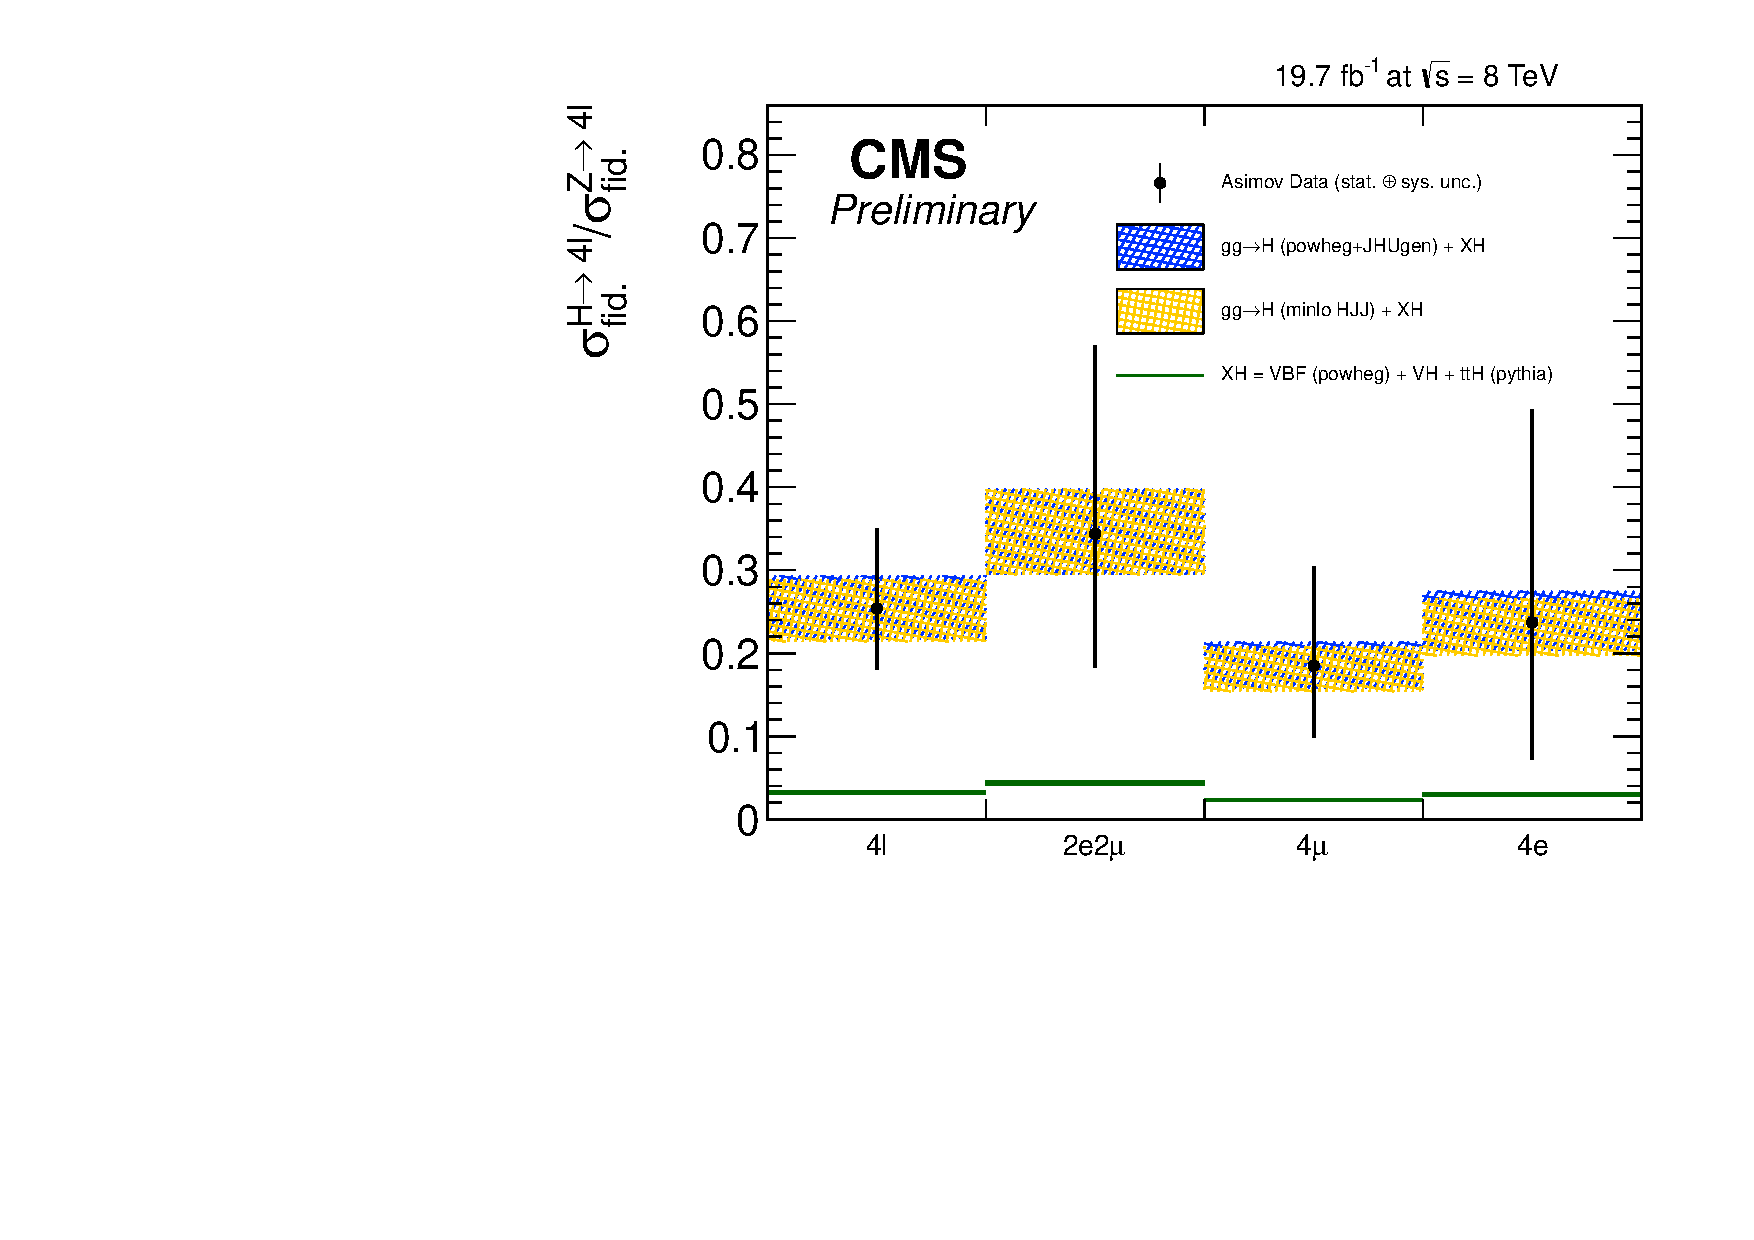
\includegraphics[width=0.65\textwidth,angle=0]{Appendix/Plots/ratio_Ratio_SM_125_mass4l_Asimov_floatPOIs_fixMH_fixDeltaMHmZ_all_8TeV_xs_v1_v2.pdf}
    \caption{Results of inclusive fiducial cross section of H$\rightarrow 4l$ and Z$\rightarrow 4l$ for different final states, obtained
from a simultaneous fit of mass peaks of Z$\rightarrow 4l$ and H$\rightarrow 4l$ (Asimov dataset) in mass window 50 to 140 GeV.
    COMMENT: Results shown with Asimov dataset.
} 
  \label{fig:inclusive-results-simfit-asimov}
 \end{center}
\end{figure}

%============
\begin{table}[!h!tb]
\begin{center}
      \caption{
Ratio of inclusive fiducial cross section of H$\rightarrow 4l$ and Z$\rightarrow 4l$, obtained
from a simultaneous fit of mass peaks of Z$\rightarrow 4l$ and H$\rightarrow 4l$ (Asimov dataset) in mass window 50 to 140 GeV.
    COMMENT: Results shown with Asimov dataset.
        } \label{tab:incresults-simfit-asimov}
\begin{tabular}{|c|c|}
\hline %---------------------------------------------------------
\hline %---------------------------------------------------------
\multicolumn{2}{|c|}{ ratio of fiducial cross sections of H$\rightarrow 4l$ and Z$\rightarrow 4l$} \\
\multicolumn{2}{|c|}{($50~GeV < m_{4\ell} < 140~GeV$)} \\
\hline %---------------------------------------------------------
\vspace{-0.4cm} & \\
Measured & $0.254^{+0.096}_{-0.074}({\rm stat.}\oplus{\rm sys.})$  \\
\vspace{-0.4cm} & \\
\hline %---------------------------------------------------------
\vspace{-0.4cm} & \\
\small gg$\rightarrow$H({\sc pohwheg+JHUgen}) + XH and Z$\rightarrow 4l$ ({\sc powheg}) & $ 0.254^{+0.040}_{-0.036}$ \\
\hline %---------------------------------------------------------
\vspace{-0.4cm} & \\
\small gg$\rightarrow$H({\sc minloHJJ}) + XH and Z$\rightarrow 4l$ ({\sc powheg}) & $ 0.249^{+0.039}_{-0.036}~$ \\
\hline %---------------------------------------------------------
\hline %---------------------------------------------------------
\end{tabular}
\end{center}
\end{table}
%============

%7/8 ratio
\begin{figure}[!h!tb]
  \begin{center}
      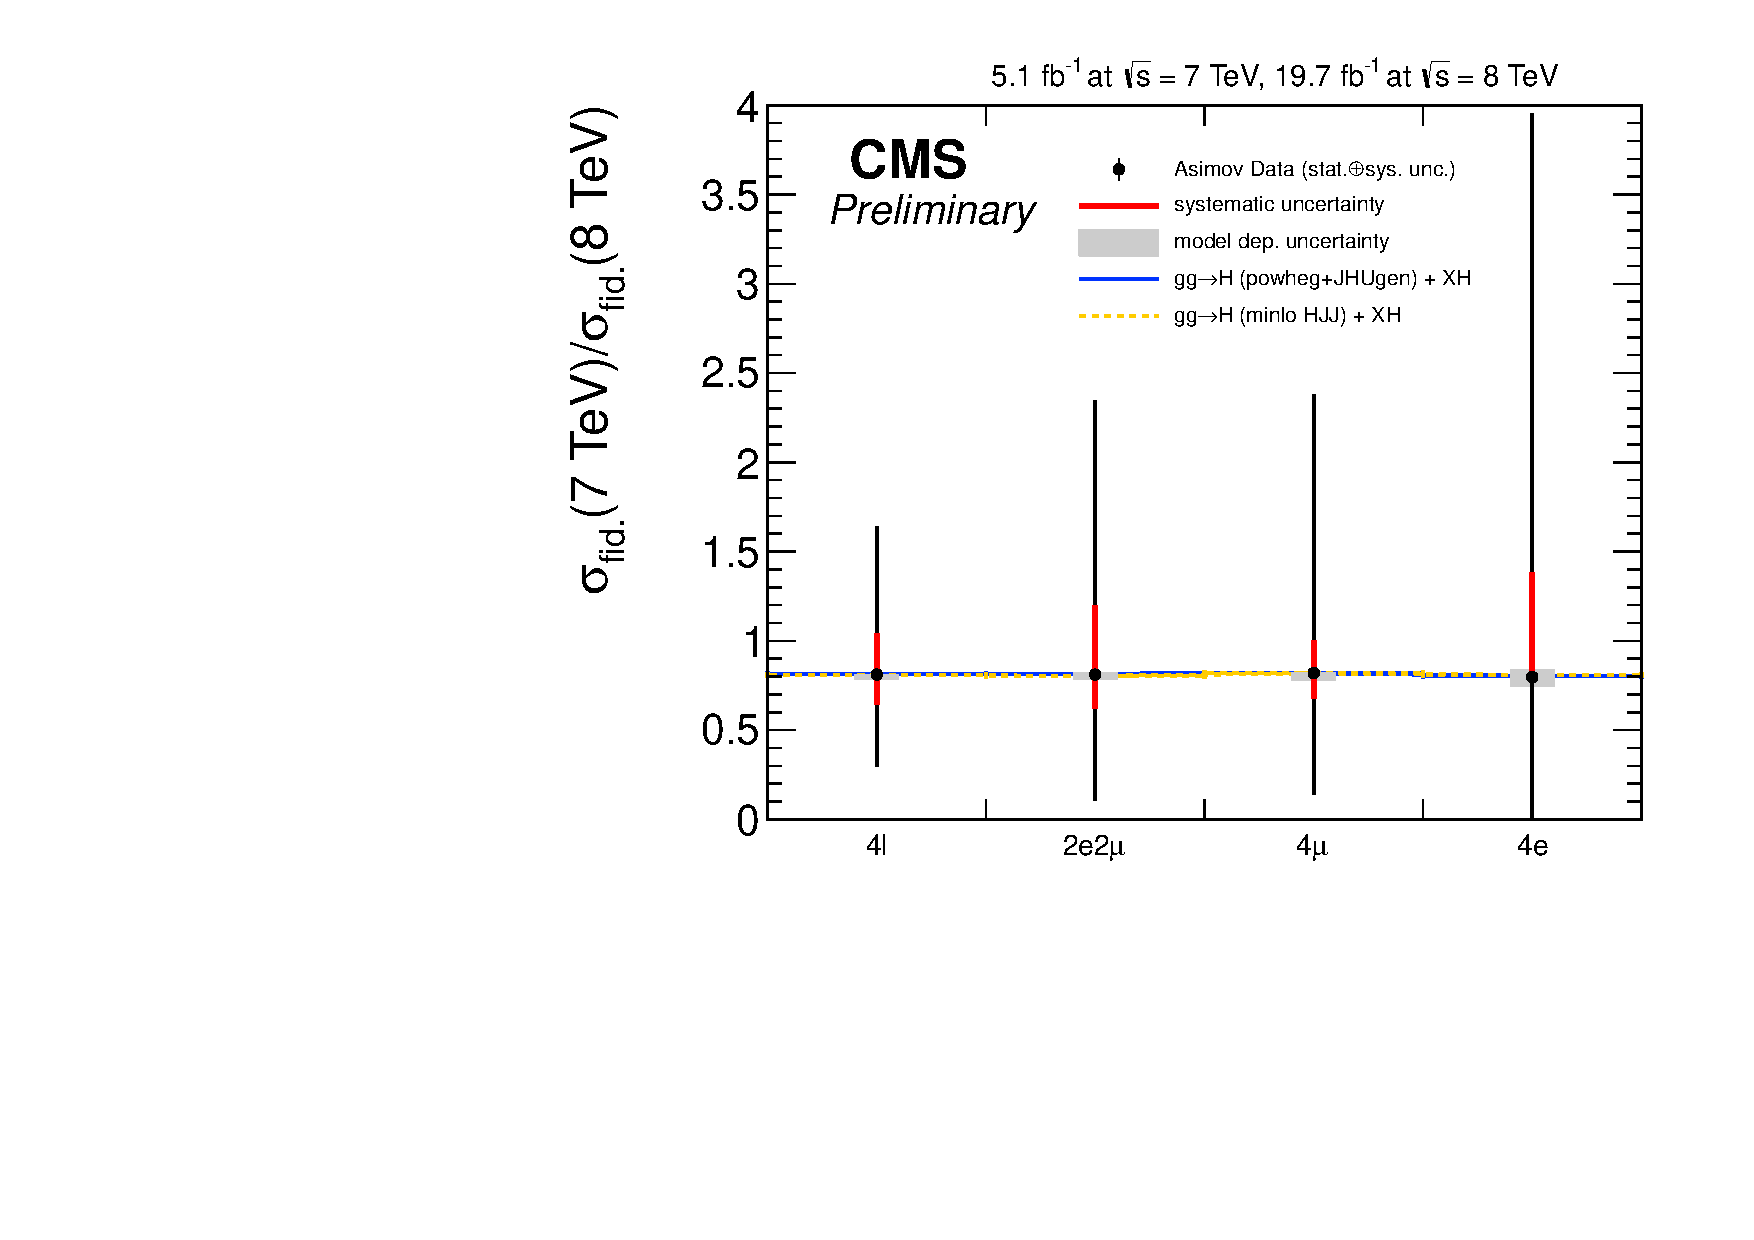
\includegraphics[width=0.65\textwidth,angle=0]{Appendix/Plots/ratio7to8_mass4l_unfoldwith_SM_125.pdf}
    \caption{Ratio of inclusive fiducial cross section of H$\rightarrow 4l$ at 7 and 8~TeV for different final states, obtained
from a simultaneous fit of mass peaks of H$\rightarrow 4l$ (Asimov dataset) in 7 and 8~TeV dataset in mass window 105 to 140 GeV.
    COMMENT: Results shown with Asimov dataset.
} 
  \label{fig:inclusive-ratio7o8-asimov}
 \end{center}
\end{figure}




%============
\begin{table}[!h!tb]
\begin{center}
      \caption{
Ratio of inclusive fiducial cross section of H$\rightarrow 4l$ and Z$\rightarrow 4l$, obtained
from a simultaneous fit of mass peaks of Z$\rightarrow 4l$ and H$\rightarrow 4l$ (Asimov dataset) in mass window 50 to 140 GeV.
    COMMENT: Results shown with Asimov dataset.
        } \label{tab:incresults-simfit-asimov}
\begin{tabular}{|c|c|}
\hline %---------------------------------------------------------
\hline %---------------------------------------------------------
\multicolumn{2}{|c|}{ ratio of fiducial cross sections of H$\rightarrow 4l$ at 7 and 8~TeV} \\
%\multicolumn{2}{|c|}{($105~GeV < m_{4\ell} < 140~GeV$)} \\
\hline %---------------------------------------------------------
\vspace{-0.4cm} & \\
Measured & $0.811^{\rm +0.837}_{\rm -0.509} \, {\rm(stat.)}\, ^{\rm +0.312}_{\rm -0.110}\,  {\rm (sys.)} \, ^{+0.000}_{-0.029}\,  {\rm (model)}\,$  \\
\vspace{-0.4cm} & \\
\hline %---------------------------------------------------------
\vspace{-0.4cm} & \\
\small gg$\rightarrow$H({\sc powheg+JHUgen}) + XH & $0.814$ \\
\hline %---------------------------------------------------------
\vspace{-0.4cm} & \\
\small gg$\rightarrow$H({\sc minloHJJ}) + XH & $0.809$ \\
\hline %---------------------------------------------------------
\hline %---------------------------------------------------------
\end{tabular}
\end{center}
\end{table}
